\documentclass[xcolor=svgnames,dvipsnames,table, hyperref=pdftex, mathserif, presentation]{beamer}
\usepackage{amsmath,amssymb,amsfonts,amsthm}
\usepackage{ctex}
\setCJKsansfont{KaiTi}% 文泉驿的黑体
\usepackage{graphics}
\usepackage{graphicx}
\usepackage{xcolor}
\usepackage{wasysym}
\usepackage{bbm}
\usepackage{url}
\usepackage{beamerleanprogress}
\usepackage{tikz-dependency}
\usepackage{tikz-qtree}
\usepackage{multirow}

% for uml charts
\usepackage{tikz}
\usetikzlibrary{calc,arrows.meta, graphs, trees, shapes, positioning, automata,
shapes.geometric, shapes.multipart, er, patterns, decorations.markings, intersections, decorations.text}
\usepackage{tikz-uml}

% for overlap pictures
\usepackage{overpic}

% for customize itemize
% \usepackage{lipsum}
% \usepackage{paralist}
% \setbeamertemplate{itemize/enumerate body begin}{\large}
% \setbeamertemplate{itemize/enumerate subbody begin}{\tiny}


\newcommand{\tabincell}[2]{\begin{tabular}{@{}#1@{}}#2\end{tabular}}%放在导言区
\usetheme{CambridgeUS}
%\usetheme{Pittsburgh}
\usecolortheme{orchid} % seahorse  orchid rose
\setbeamertemplate{blocks}[rounded][shadow=true]
\AtBeginSection[]{%
  \begin{frame}<beamer>
    \frametitle{Outline}
      \tableofcontents[current] 
    \end{frame}
  \addtocounter{framenumber}{-1}% If you don't want them to affect the slide number
}
\AtBeginSubsection[]
{
  \begin{frame}
  \frametitle{Outline}
    \tableofcontents[currentsection,currentsubsection]
  %\tableofcontents[sectionstyle=show/hide,subsectionstyle=hide/show/hide]
  \end{frame}
  \addtocounter{framenumber}{-1}% If you don't want them to affect the slide number
}
\newcommand{\setof}[1]{\ensuremath{\left \{ #1 \right \}}}
\newcommand{\tuple}[1]{\ensuremath{\left \langle #1 \right \rangle }}
\newcommand{\red}[1]{\textcolor{red}{#1}}
\newcommand{\brown}[1]{\textcolor{brown}{#1}}
\newcommand{\green}[1]{\textcolor{green}{#1}}
\newcommand{\blue}[1]{\textcolor{blue}{#1}}
\newcommand{\cyan}[1]{\textcolor{cyan}{#1}}

%gets rid of navigation symbols
\setbeamertemplate{navigation symbols}{}

\begin{document}
 
\title[LOD-synonym]{利用关联规则在结构化三元组中查找相同语义的谓词\\
}
\subtitle{Synonym Analysis for Predicate Expansion \\ eswc2013}

\institute[icst@pku]{
  hanzhe@icst-wip
}
\author[Zhe Han]{\\ 
Ziawasch Abedjan @hpi.de \begin{footnotesize}哈索·普拉特纳研究院\end{footnotesize}\\
Felix Naumann@hpi.de\\
}

\frame[t,plain]{ \titlepage } % [t,plain]

\frame{
  \frametitle{ Outline  }
  
   \begin{itemize}
    \item summary
      \begin{itemize}
       \item 论文动机
	\begin{itemize}
	 \item 找到LOD(linked-open-data)里面重复的谓词
	\end{itemize}
       \item 方法概述
	\begin{itemize}
	 \item 将谓词加到关联规则中,挖掘相同的谓词对
	\end{itemize}
       \item dbpedia实验效果
      \end{itemize}
   \end{itemize}

}

\frame{
  \frametitle{关联规则}
  \begin{block}{}
   \begin{itemize}
    \item 项集(item set):$I=\{i_1,i_2,...,i_m\}$
    \item 事务集(Transaction set):$T=\{t|t\subseteq I\}$
    \item 一个关联规则$X\to Y$, 其中 $X,Y\subseteq I, X\cap Y=\emptyset$
      \begin{itemize}
       \item 该关联规则的支持度(support):$\frac{|\{t|t\in T, X\cup Y\subseteq t\}|}{|T|}$
       \item 该关联规则的置信度(confidence):$\frac{|\{t|t\in T,  X\cup Y\subseteq t\}|}{|\{t|t\in T, X\subseteq t\}|}$
      \end{itemize}
      
   \end{itemize}
  \end{block}
}

\frame{
  \frametitle{关联规则}

  \begin{center}
   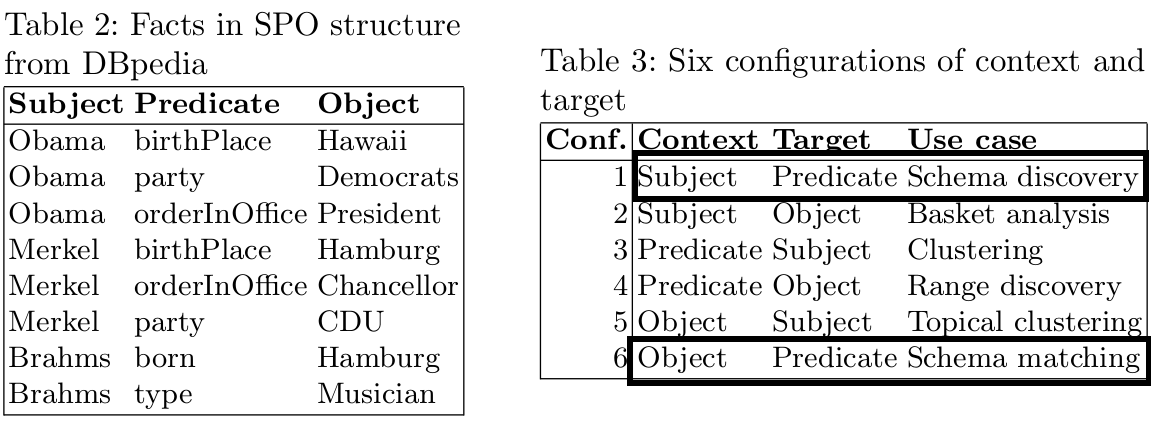
\includegraphics[width=0.9\hsize]{pic/method.png}
  \end{center}
  \begin{columns}
   \column{0.4\hsize}
    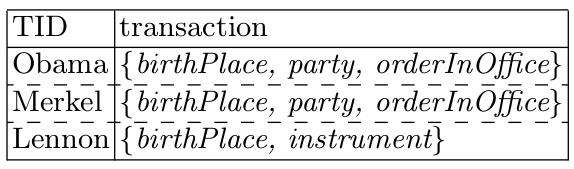
\includegraphics[width=0.9\hsize]{pic/f1.png}
   \column{0.5\hsize}
    \begin{itemize}
     \item $birthPlace\to orderInOffice$ 置信度66.7\%,支持度66.7\%, $orderInOffice\to birhtPlace$置信度100\%,支持度66.7\%
    \end{itemize}
   
  \end{columns}

}


\frame{
  \begin{columns}[c]
   \column{.15\hsize}
   \column{.7\hsize}
   \begin{block}{}
    \centering \Large 方法说明 \\ 
    \small --- 
   \end{block}

   \column{.15\hsize}
  \end{columns}

}


\frame{
  \frametitle{方法说明}
  如果谓词$p_1,p_2$意义相同,则:
  \begin{enumerate}
   \item 他们不会出现在同一个主语的谓词集合里
   \item 他们所在的三元组含有很多相同的客体
   \item 他们所在的三元组的客体类别的分布很相似
  \end{enumerate}
}

\frame{
  \frametitle{方法说明}
   如果谓词$p_1,p_2$意义相同
    \begin{enumerate}
%      \setcounter{enumi}{2}
     \item 他们不会出现在同一个主语的谓词集合里(RCC)
    \end{enumerate}
  
  \begin{center}
   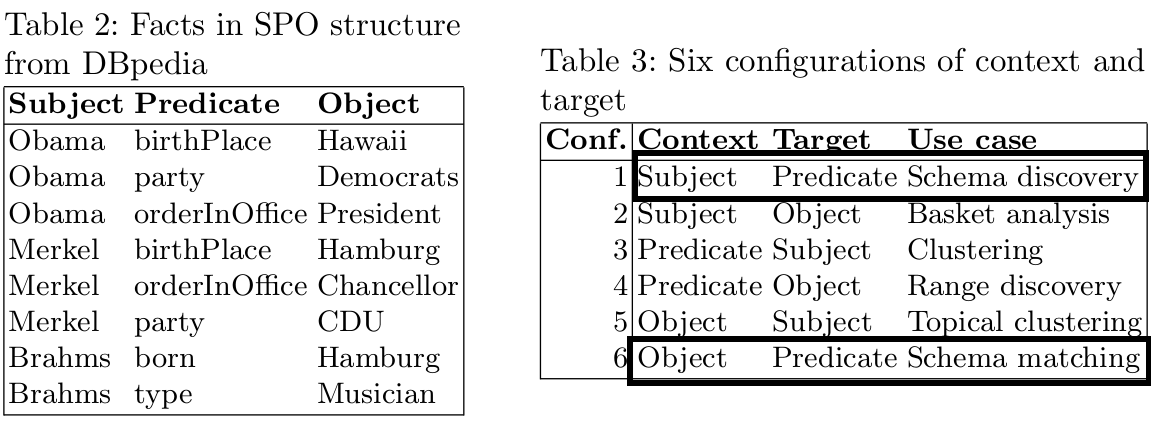
\includegraphics[width=0.7\hsize]{pic/method.png}
  \end{center}
  \begin{columns}
   \column{0.4\hsize}
    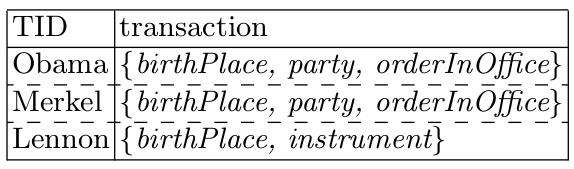
\includegraphics[width=0.9\hsize]{pic/f1.png}
   \column{0.5\hsize}
    \begin{itemize}\begin{footnotesize}
     \item $X\to\neg Y$,$Y\to\neg X$置信度都很高(避免Y出现频率很低造成$X\to\neg Y$)
     \only<1>{\item 比如$party\to\neg instrument$, $birthPlace\to\neg born$}
     \end{footnotesize}
    \end{itemize}
  \end{columns}
     \only<2>{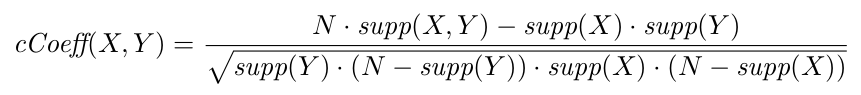
\includegraphics[width=0.9\hsize]{pic/RCC.png}}
  
}

\frame{
  \frametitle{方法说明}
  如果谓词$p_1,p_2$意义相同
  \begin{large}
   \begin{center}
    \begin{enumerate}
     \setcounter{enumi}{1}\begin{footnotesize}
     \item 他们所在的三元组含有很多相同的客体(RCF-range content filtering)
     \end{footnotesize}
    \end{enumerate}
   \end{center}
  \end{large}

  \begin{center}
   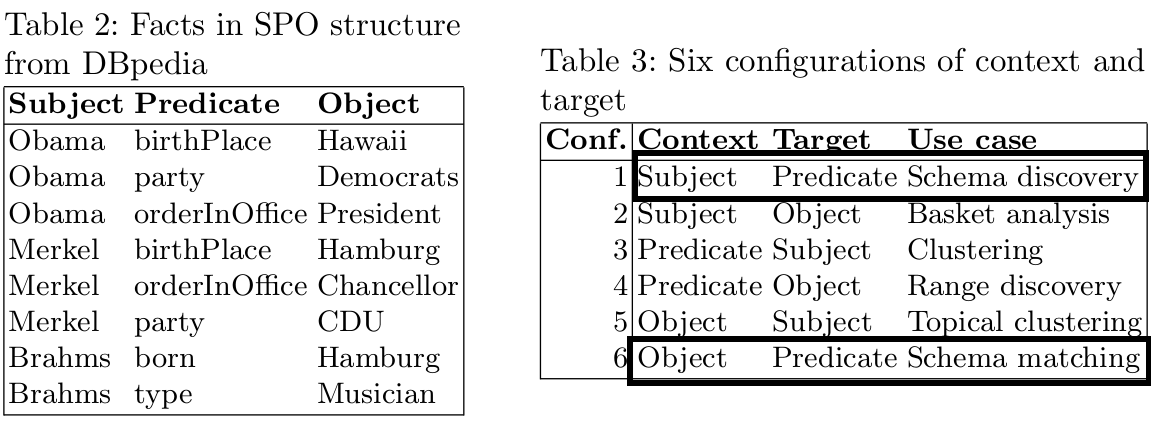
\includegraphics[width=0.7\hsize]{pic/method.png}
  \end{center}
  \begin{columns}
   \column{0.4\hsize}
    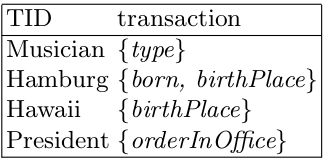
\includegraphics[width=0.9\hsize]{pic/RCF.png}
   \column{0.5\hsize}
    \begin{itemize}\begin{footnotesize}
     \item $born$和$birthPlace$
     \only<1>{\item 比如$party\to\neg instrument$, $birthPlace\to\neg born$}
     \end{footnotesize}
    \end{itemize}
  \end{columns}
}

\frame{
  \frametitle{方法说明}
  如果谓词$p_1,p_2$意义相同
   \begin{center}
    \begin{enumerate}
     \setcounter{enumi}{2}
     \item 他们所在的三元组含有很多相同的客体(RSF-range Structure/type filtering)
    \end{enumerate}
   \end{center}

  类似range content filtering,将content用对应类别替代,计算任意一个谓词对$p_1,p_2$,只需要计算类别向量的相似度
}


\frame{
  \frametitle{方法说明}
  如果谓词$p_1,p_2$意义相同,则前面3种想法\red{混合}:
  \begin{enumerate}
   \item 根据(RCF-range content filtering)得到所有的谓词对候选(每对谓词至少重复一个客体)
   \item 根据(RSF-range Structure/type filtering)进一步筛选谓词对(每对谓词至少有一个相同的客体类别)
    \begin{itemize}
     \item 第一阶段可以重复的客体可能是数值或时间(没有类别),不算相同的可以类别
    \end{itemize}
   \item 使用不同的评价标注(RCC/minConf/maxConf/...)计算每个谓词对的相似度
  \end{enumerate}
}

\frame{
  \begin{columns}[c]
   \column{.15\hsize}
   \column{.7\hsize}
   \begin{block}{}
    \centering \Large 实验 \\ 
    \small --- 
   \end{block}

   \column{.15\hsize}
  \end{columns}

}

\frame{
  \only<1>{\frametitle{实验一}}
  \only<2>{\frametitle{实验二}}
  \only<3>{\frametitle{实验三}}
  
  \only<1>{
    \begin{columns}
     \column{0.6\hsize}
    \begin{itemize}
     \item 比较使用客体类别向量/客体值来判断为此对相似性
     \only<2>{\item type不好是因为作者没有考虑所有数值型谓词,作者认为他们没有类别,相似性就是0}
    \end{itemize}
     \column{0.4\hsize}
     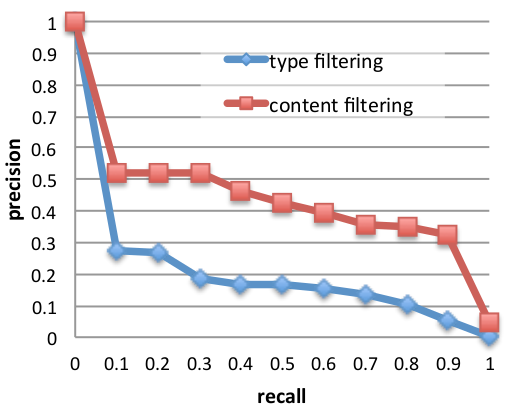
\includegraphics[width=0.9\hsize]{pic/exp1.png}
    \end{columns}
  }
  \only<2>{
    \begin{columns}
     \column{0.4\hsize}
     \begin{itemize}\begin{small}
     \item syn是别人的方法:相同的谓词不共现、含有相似客体
      \item minConf, maxConf, fmeasure与RCC类似
	 \item 希望利用“$X\to \neg Y$是一个频繁模式”来表达两个相同的谓词
	 \item minConf=$min\{conf(X\to \neg Y), conf(Y\to\neg X)\}$
	 \item maxCont=$max\{...\}$
	 \item fmeasur是$minCont$和$maxCont$的调和平均数
      \end{small}
     \end{itemize}
     \column{0.6\hsize}
  \begin{block}{}
   抽取在dbpedia `Work`(作品)类别下的9456个谓词对,其中82对意思相同
  \end{block}
  \vspace{1cm}
     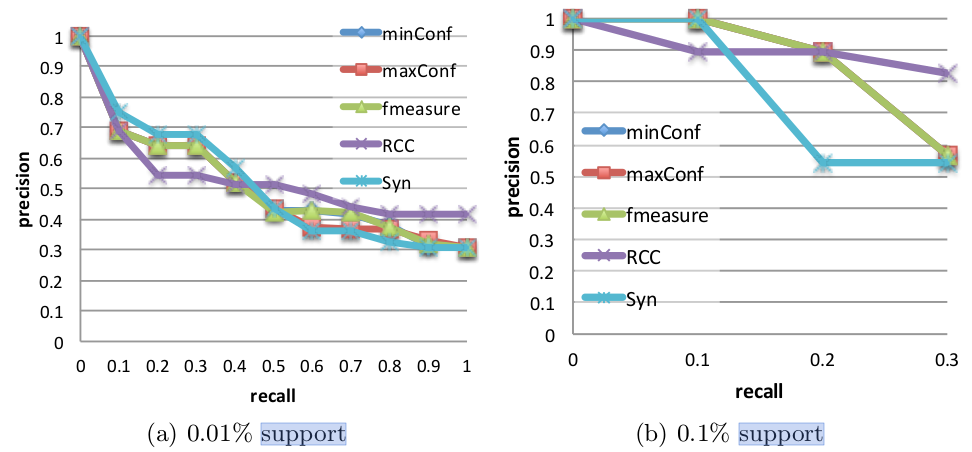
\includegraphics[width=1.0\hsize]{pic/rcc-exp.png}

    \end{columns}
    \begin{itemize}
     \item RCC= 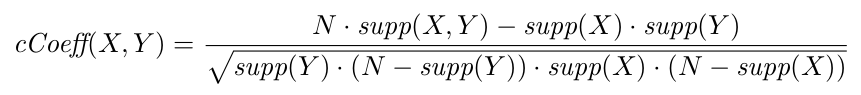
\includegraphics[width=0.7\hsize]{pic/RCC.png}
    \end{itemize}
  }
  
  \only<3>{
    通过RCF对谓词对进行过滤的效果
  \begin{center}
   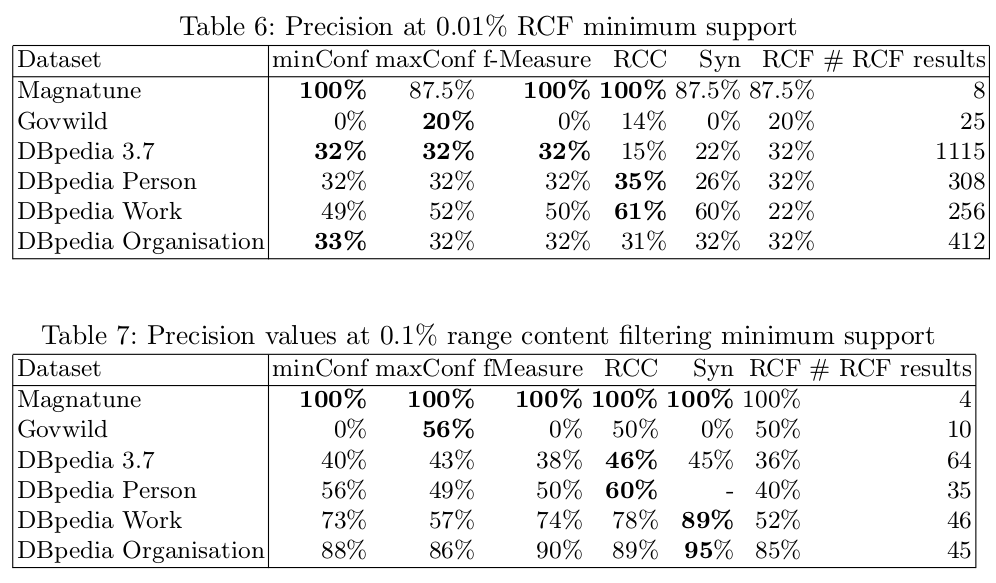
\includegraphics[width=0.7\hsize]{pic/rcf-exp.png}
  \end{center}
    \begin{itemize}
     \item 上下两个图对比,可以发现RCf过滤有用
     \item 上图的Dbpedia work数据集49\%的准确率比实验二的30\%左右的准确率高出不少
    \end{itemize}

  }
}
\frame{
  \begin{center}
   \Large 谢谢大家
   
  \end{center}

}

\end{document}

